\section{$G$-cr vs $G$-cr over $k$ (Proof of Theorem~\ref{D4example})}
Let $G$ be a simple algebraic group of type $D_4$ defined over a nonperfect field $k$ of characteristic $2$. Fix a maximal $k$-torus of $G$ and a $k$-defined Borel subgroup of $G$. let $\Psi(G)=\Psi(G,T)$ be the set of roots corresponding to $T$, and $\Psi(G)^{+}=\Psi(G,B,T)$ be the set of positive roots of $G$ corresponding to $T$ and $B$. The following Dynkin diagram defines the set of simple roots of $G$.
\begin{figure}[h]
                \centering
                \scalebox{0.7}{
                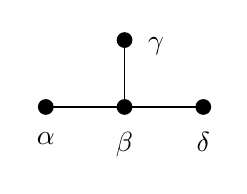
\begin{tikzpicture}
                \draw (1,0) to (2,0);
                \draw (2,0) to (2,0.85);
                \draw (2,0) to (3,0);
                \fill (1,0) circle (1mm);
                \fill (2,0) circle (1mm);
                \fill (2,0.85) circle (1mm);
                \fill (3,0) circle (1mm);
                \draw[below] (1,-0.2) node{$\alpha$};
                \draw[below] (2,-0.2) node{$\beta$};
                \draw[below] (2.4,1) node{$\gamma$};
                \draw[below] (3,-0.2) node{$\delta$};
               \end{tikzpicture}}
\end{figure}

We label $\Psi(G)^{+}$ in the following. The corresponding negative roos are defined accordingly. Note that Roots 1, 2, 3, 4 correspond to $\alpha$, $\gamma$, $\delta$, $\beta$ respectively.
\begin{table}[!h]
\begin{center}
\scalebox{0.7}{
\begin{tabular}{cccccc}
\rootsD{1}{0}{1}{0}{0}&\rootsD{2}{1}{0}{0}{0}&\rootsD{3}{0}{0}{0}{1}&\rootsD{4}{0}{0}{1}{0}&\rootsD{5}{0}{1}{1}{0}&\rootsD{6}{1}{0}{1}{0}\\
\rootsD{7}{0}{0}{1}{1}&\rootsD{8}{1}{1}{1}{0}&\rootsD{9}{0}{1}{1}{1}&\rootsD{10}{1}{0}{1}{1}&\rootsD{11}{1}{1}{1}{1}&\rootsD{12}{1}{1}{2}{1}\\
\end{tabular}
}
\end{center}
\end{table}   
Let
$\lambda:=(\alpha+2\beta+\gamma+\delta)^{\vee}=\alpha^{\vee}+2\beta^{\vee}+\gamma^{\vee}+\delta^{\vee}$. 
Then 
$
P_\lambda=\langle T, U_{\zeta}\mid \zeta\in \Psi(G)^{+}\cup \{-1,-2,-3\} \rangle,
L_\lambda=\langle T, U_{\zeta}\mid \zeta\in \{\pm 1,\pm 2,\pm 3\} \rangle,
R_u(P_\lambda)=\langle U_{\zeta} \mid \zeta \in \Psi(G)^{+}\backslash \{1, 2, 3\} \rangle.
$
Let $a\in k\backslash k^2$. Pick $b\in k^{*}$ with $b^3=1$ and $b\neq 1$. Let $v(\sqrt a):=\epsilon_{4}(\sqrt a)\epsilon_{11}(\sqrt a)\in R_u(P_\lambda)(\overline k)$. Define
\begin{equation*}
H:=v(\sqrt a)\cdot\langle n_\alpha n_\gamma n_\delta, \; (\alpha+\gamma+\delta)^{\vee}(b) \rangle.
\end{equation*}
Here is our first main result in this section.
\begin{prop}\label{firstmain}
$H$ is $k$-defined. Moreover, $H$ is $G$-cr but not $G$-cr over $k$. 
\end{prop}
\begin{proof}
First, we have 
$
(n_\alpha n_\gamma n_\delta) \cdot (\beta) = (n_\alpha n_\gamma n_\delta) \cdot 4 = 11, \;
(n_\alpha n_\gamma n_\delta) \cdot 11 = 4.
$
Using this and the commutation relations~\cite[Lem.~32.5 and Prop.~33.3]{Humphreys-book1}, we obtain
\begin{equation*}
v(\sqrt a)\cdot (n_{\alpha} n_\gamma n_\delta)=(n_\alpha n_\gamma n_\delta) \epsilon_{12}(a).
\end{equation*}
Since $\langle 4, (\alpha+\gamma+\delta)^{\vee}\rangle=-3$, $\langle 11, (\alpha+\gamma+\delta)^{\vee}\rangle=3$, and $b^3=1$, $v(\sqrt a)$ commutes with $(\alpha+\gamma+\delta)^{\vee}(b)$. Now it is clear that $H$ is $k$-defined (since it is generated by $k$-points). 

Now we show that $H$ is $G$-cr. It is sufficient to show that $H':=v(\sqrt a)^{-1}\cdot H=\langle n_\alpha n_\gamma n_\delta,\; (\alpha+\gamma+\delta)^{\vee}(b)$ is $G$-cr since it is $G$-conjugate to $H$. Since $H'$ is contained in $L_\lambda$, by Proposition~\ref{G-cr-L-cr} it is enough to show that $H'$ is $L_\lambda$-cr. By inspection, $H'$ is $L_\lambda$-ir (this is easy since $L_\lambda=L_\alpha\times L_\gamma\times L_\delta=A_1\times A_1 \times A_1$). 


Next, we show that $H$ is not $G$-cr over $k$. Suppose the contrary. Clearly $H$ is contained in $P_\lambda$ that is $k$-defined. Then there exists a $k$-defined Levi subgroup of $P_\lambda$ containing $H$. Then by~\cite[Lem.~2.5(\rmnum{3})]{Bate-uniform-TransAMS} there exists $u\in R_u(P_\lambda)(k)$ such that $H$ is contained in $u\cdot L_\lambda$. Thus $n_\alpha n_\gamma n_\delta \epsilon_{12}(a) < u\cdot L_\lambda$. So $u^{-1}\cdot (n_\alpha n_\gamma n_\delta \epsilon_{12}(a)) < L_{\lambda}$. By~\cite[Prop.~8.2.1]{Springer-book}, we set
$
u:=\prod_{\zeta\in \Psi(R_u(P_\lambda))}\epsilon_\zeta(x_\zeta).
$
Using the labelling of the positive roots above, we have $\Psi(R_u(P_\lambda))=\{4,\cdots 12\}$. We compute how $n_\alpha n_\gamma n_\delta$ acts on $\Psi(R_u(P_\lambda))$: 
\begin{equation}\label{perm}
n_\alpha n_\gamma n_\delta = (4\;11) (5\;10) (6\;9) (7\;8) (12). 
\end{equation}
Using this and the commutation relations,
\begin{alignat*}{2}
u^{-1}\cdot (n_\alpha n_\gamma n_\delta \epsilon_{12}(a))
=&n_\alpha n_\gamma n_\delta \epsilon_4(x_4+x_{11})\epsilon_{5}(x_5+x_{10})\epsilon_{6}(x_6+x_9)\epsilon_{7}(x_{7}+x_{8})\\
&\epsilon_{8}(x_7+x_8)\epsilon_{9}(x_6+x_{9})\epsilon_{10}(x_5+x_{10})\epsilon_{11}(x_4+x_{11})\\
&\epsilon_{12}(x_{4}^2+x_{5}^2+x_{6}^2+x_{7}^2 +a).
\end{alignat*}
Thus if $u^{-1}\cdot (n_\alpha\sigma \epsilon_{\alpha+2\beta+\gamma+\delta}(a)) < L_{\lambda}$ we must have
\begin{equation*}
x_4=x_{11},\; x_5=x_{10},\; x_{6}=x_{9},\; x_7=x_8,\; x_{4}^2+ x_{5}^2+x_{6}^2+x_{7}^2 +a=0.
\end{equation*}
The last equation gives $(x_4+x_5+x_6+x_7)^2=a$. This is impossible since $a\notin k^2$. We are done. 
\end{proof}

\begin{rem}\label{D4nonsep}
From the computations above we see that the curve $C(x):=\{\epsilon_{4}(x)\epsilon_{11}(x)\mid x\in \overline k\}$ is not contained in $C_G(H)$, but the corresponding element in $\textup{Lie}(G)$, that is, $e_4+e_{11}$ is contained in $\mathfrak{c}_{\mathfrak{g}}(H)$. Then the argument in the proof of~\cite[Prop.~3.3]{Uchiyama-Separability-JAlgebra} shows that $\textup{Dim}(C_G(H))$ is strictly smaller than $\textup{Dim}(\mathfrak{c}_{\mathfrak{g}}(H))$. So $H$ is non-separable in $G$. 
In fact, combining~\cite[Thm.~1.5]{Bate-cocharacter-Arx} and~\cite[Thm.~9.3]{Bate-cocharacter-Arx} we have that if a $k$-subgroup $H$ of $G$ is separable in $G$ and $H$ is $G$-cr, then it is $G$-cr over $k$. 
\end{rem}

\vspace{5mm}
Now we move on to the second main result in this section. We use the same $k$, $a$, $b$, $G$, and, $\lambda$ as above. Let $v(\sqrt a):=\epsilon_{-11}(\sqrt a)\epsilon_{-4}(\sqrt a)$. Let
\begin{equation*}
K:=v(\sqrt a)\cdot \langle n_{\alpha} n_{\gamma} n_{\delta},\; (\alpha+\gamma+\delta)^{\vee}(b)\rangle=\langle n_\alpha n_\gamma n_\delta \epsilon_{-12}(a), \;  (\alpha+\gamma+\delta)^{\vee}(b)\rangle. 
\end{equation*}
Define
\begin{equation*}
H:=\langle K, \; \epsilon_{5}(1) \rangle.
\end{equation*}

\begin{prop}\label{secondmain}
$H$ is $k$-defined. Moreover, $H$ is $G$-ir over $k$ but not $G$-cr. 
\end{prop}
\begin{proof}
$H$ is clearly $k$-defined. First, we show that $H$ is $G$-ir over $k$. Note that
\begin{equation*}
v(\sqrt a)^{-1}\cdot H = \langle n_\alpha n_\gamma n_\delta, \; (\alpha+\gamma+\delta)^{\vee}(b),\; \epsilon_{5}(1)\epsilon_{1}(\sqrt a)\rangle.
\end{equation*}
Thus we see that $v(\sqrt a)^{-1}\cdot H$ is contained in $P_\lambda$. So $H$ is contained in $v(\sqrt a)\cdot P_\lambda$. 

\begin{lem}\label{uniquepara}
$v(\sqrt a)\cdot P_\lambda$ is the unique proper parabolic subgroup of $G$ containing $H$.
\end{lem}
\begin{proof}
Suppose that $P_\mu$ is a proper parabolic subgroup of $G$ containing $v(\sqrt a)^{-1}\cdot H$. In the proof of Proposition~\ref{firstmain} we have shown that $M:=\langle n_\alpha n_\gamma n_\delta, (\alpha+\gamma+\delta)^{\vee}(b)\rangle$ is $G$-cr. Then there exists a Levi subgroup $L$ of $P_\mu$ containing $M$ since $M$ is contained in $P_\mu$. Since Levi subgroups of $P_\mu$ are $R_u(P_\mu)$-conjugate by~\cite[Lem.~2.5(\rmnum{3})]{Bate-uniform-TransAMS}, without loss, we set $L:=L_\mu$. Then $M<L_\mu=C_G(\mu(\overline k^*))$, so $\mu(\overline k^*)$ centralizes $M$. Recall that by~\cite[Thm.~13.4.2]{Springer-book}, $C_{R_u(P_\lambda)}(M)^{\circ}\times C_{L_\lambda}(M)^{\circ}\times C_{R_u(P_\lambda^{-})}(M)^{\circ}$ is an open set of $C_G(M)^{\circ}$ where $P_\lambda^{-}$ is the opposite of $P_\lambda$ containing $L_\lambda$.  
\begin{lem}\label{centralizerofM}
$C_G(M)^{\circ}=G_{12}$.
\end{lem}
\begin{proof}
First of all, from Equation~(\ref{perm}) we see that $G_{12}$ is contained in $C_G(n_\alpha n_\gamma n_\delta)$. Since $\langle 12, (\alpha+\gamma+\delta)^{\vee} \rangle=0$, $G_{12}$ is also contained in $C_G((\alpha+\gamma+\delta)^{\vee}(\overline k^*))$. So $G_{12}$ is contained in $C_G(M)$. Set $u:=\prod_{i\in \Psi(R_u(P_\lambda))}\epsilon_{i}(x_i)$ for some $x_i \in \overline k$. Using Equation (\ref{perm}) and the commutation relations, we obtain
\begin{alignat*}{2}
(n_\alpha n_\gamma n_\delta)\cdot u =& \epsilon_{4}(x_{11})\epsilon_{5}(x_{10})\epsilon_{6}(x_9)\epsilon_7(x_{8})\epsilon_8(x_{7})\epsilon_9(x_6)\epsilon_{10}(x_{5})\epsilon_{11}(x_4)\\
&\epsilon_{12}(x_4 x_{11}+x_5 x_{10} +x_6 x_9+ x_7 x_8+ x_{12}). 
\end{alignat*}
So, if $u\in C_{R_u(P_\lambda)}(n_\alpha n_\gamma n_\delta)$ we must have
$x_4=x_{11}, \; x_5=x_{10},\; x_{6}=x_{9},\; x_7=x_8$, and $x_4 x_{11}+x_5 x_{10} +x_6 x_9+ x_7 x_8=0$. But $\langle \zeta, (\alpha+\gamma+\delta)^{\vee}\rangle=-1$ for $\zeta=\{5, 6, 7\}$, so $x_5=x_6=x_7=0$ for $u\in C_{R_u(P_\lambda)}(M)$. Then 
\begin{equation*}
(n_\alpha n_\gamma n_\delta)\cdot u = \epsilon_4(x_4)\epsilon_{11}(x_4)\epsilon_{12}(x_4^2+x_{12}).
\end{equation*}
So we must have $x_4^2=0$ if $u\in C_{R_u(P_\lambda)}(M)$. Thus we conclude that $C_{R_u(P_\lambda)}(M)=U_{12}$. Similarly, we can show that $C_{R_u(P_{\lambda}^{-})}(M)=U_{-12}$. A direct computation shows that $C_{L_\lambda}(M) < T$ and $C_T(n_\alpha n_\gamma n_\delta)=(\alpha+2\beta+\gamma+\delta)^{\vee}(\overline k^*)<G_{12}$. We are done.
\end{proof}
Since $\mu(\overline k^*)$ centralizes $M$, Lemma~\ref{centralizerofM} yields $\mu(\overline k^*)<G_{12}$. Then we can set $\mu:=g\cdot (\alpha+2\beta+\gamma+\delta)^{\vee}$ for some $g\in G_{12}$. By the Bruhat decomposition, $g$ is one of the following forms:
\begin{alignat*}{2}
&(1)\;g=(\alpha+2\beta+\gamma+\delta)^{\vee}(s)\epsilon_{12}(x_1),\\
&(2)\;g=\epsilon_{12}(x_1)n_{12}(\alpha+2\beta+\gamma+\delta)^{\vee}(s)\epsilon_{12}(x_2)\\
&\textup{for some } x_1, x_2\in \overline k, s\in \overline k^*.
\end{alignat*}
We rule out the second case. Suppose $g$ is of the second form. Note that $\epsilon_{5}(1)\epsilon_{1}(\sqrt a)\in v(\sqrt a)^{-1}\cdot H< P_\mu$. 
But $P_\mu=P_{g\cdot (\alpha+2\beta+\gamma+\delta)^{\vee}}=g\cdot P_{(\alpha+2\beta+\gamma+\delta)^{\vee}}$. So it is enough to show that $g^{-1}\cdot (\epsilon_{5}(1)\epsilon_{1}(\sqrt a))\notin P_{(\alpha+2\beta+\gamma+\delta)^{\vee}}$. Since $U_{12}$ and $(\alpha+2\beta+\gamma+\delta)(\overline k^*)$ are contained in $P_{(\alpha+2\beta+\gamma+\delta)^{\vee}}$ we can assume $g=n_{12}$. We have
\begin{equation*}
n_{12}=n_\alpha n_\beta n_\alpha n_\gamma n_\beta n_\alpha n_\delta n_\beta n_\alpha n_\gamma n_\beta n_\delta \textup{ (the longest element in the Weyl group of $D_4$)}.
\end{equation*}
Using this, we can compute how $n_{12}$ acts on each root subgroup of $G$. In particular $n_{12}^{-1}\cdot U_{5}=U_{-5}$ and $n_{12}^{-1}\cdot U_{1}= U_{-1}$. Thus
\begin{alignat*}{2}
n_{12}^{-1}\cdot (\epsilon_{5}(1)\epsilon_{1}(\sqrt a)) &= \epsilon_{-5}(1)\epsilon_{-1}(\sqrt a)\notin P_{(\alpha+2\beta+\gamma+\delta)^{\vee}}.
\end{alignat*}
So $g$ must be of the first form. Then $g\in P_\lambda$. Thus $P_\mu=P_{g\cdot \lambda}=g\cdot P_\lambda=P_\lambda$. We are done.
\end{proof}

\begin{lem}\label{nonkdefined}
$v(\sqrt a)\cdot P_\lambda$ is not $k$-defined.
\end{lem}
\begin{proof}
Suppose the contrary. Since $P_\lambda$ is $k$-defined, $v(\sqrt a)\cdot P_\lambda$ is $G(k)$-conjugate to $P_\lambda$ by~\cite[Thm.~20.9]{Borel-AG-book}. Thus we can put $P_\lambda=g v(\sqrt a)\cdot P_\lambda$ for some $g\in G(k)$. So $g v(\sqrt a)\in P_\lambda$ since parabolic subgroups are self-normalizing. Then $g=pv(\sqrt a)^{-1}$ for some $p\in P_\lambda$. Thus $g$ is a $k$-point of $P_\lambda R_u(P_\lambda^{-})$. Then by the rational version of the Bruhat decomposition~\cite[Thm.~21.15]{Borel-AG-book}, there exists a unique $p'\in P_\lambda(k)$ and a unique $u'\in R_u(P_\lambda^{-})(k)$ such that $g=p' u'$. This is a contradiction since $v(\sqrt a)\notin R_u(P_\lambda^{-})(k)$. 
\end{proof} 
Now Lemmas~\ref{uniquepara},~\ref{nonkdefined} show that $H$ is $G$-ir over $k$. 

\begin{lem}\label{nonG-cr}
$H$ is not $G$-cr. 
\end{lem}
\begin{proof}
We had $C_G(M)^{\circ}=G_{12}$. Then $C_G(v(\sqrt a)^{-1}\cdot H)^{\circ}<G_{12}$ since $M<v(\sqrt a)^{-1}\cdot H$. Using the commutation relations, we see that $U_{12}< C_G(v(\sqrt a)^{-1}\cdot H)$. Note that $v(\sqrt a)^{-1}\cdot H$ contains $h:=\epsilon_{5}(1)\epsilon_{1}(\sqrt a)$ that does not commute with any non-trivial element of $U_{-12}$. Also, since $\langle 5, \lambda\rangle = 4$,  $h$ does not commute with any non-trivial element of $(\alpha+2\beta+\gamma+\delta)^{\vee}(\overline k^*)$.
Thus we conclude that $C_G(v(\sqrt a)^{-1}\cdot H)^{\circ}=U_{12}$. So $C_G(H)^{\circ}=v(\sqrt a)\cdot U_{12}$ which is unipotent. Then by the classical result of Borel-Tits~\cite[Prop.~3.1]{Borel-Tits-unipotent-invent}, we see that $C_G(H)^{\circ}$ is not $G$-cr.
Since $C_G(H)^{\circ}$ is a normal subgroup of $C_G(H)$, by~\cite[Ex.~5.20]{Bate-uniform-TransAMS}, $C_G(H)$ is not $G$-cr. Then by~\cite[Cor.~3.17]{Bate-geometric-Inventione}, $H$ is not $G$-cr. 
\end{proof}
\end{proof}



  